\section*{Exercice 186 -- Réglage de gain proportionnel}
\setcounter{exo}{0}

\textit{Exercices de Marc Derumaux}

On considère la FTBO dont le diagramme de Bode est tracé ci-dessous, pour une large
gamme de fréquence puis pour une gamme de fréquence plus étroite.



\begin{center}
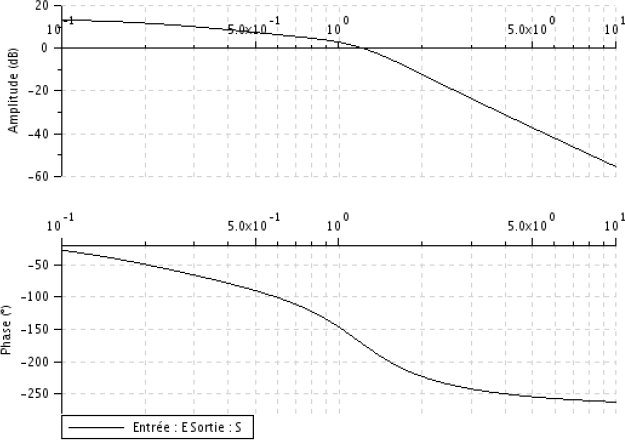
\includegraphics[width=\linewidth]{029_01}
\end{center}


\begin{center}
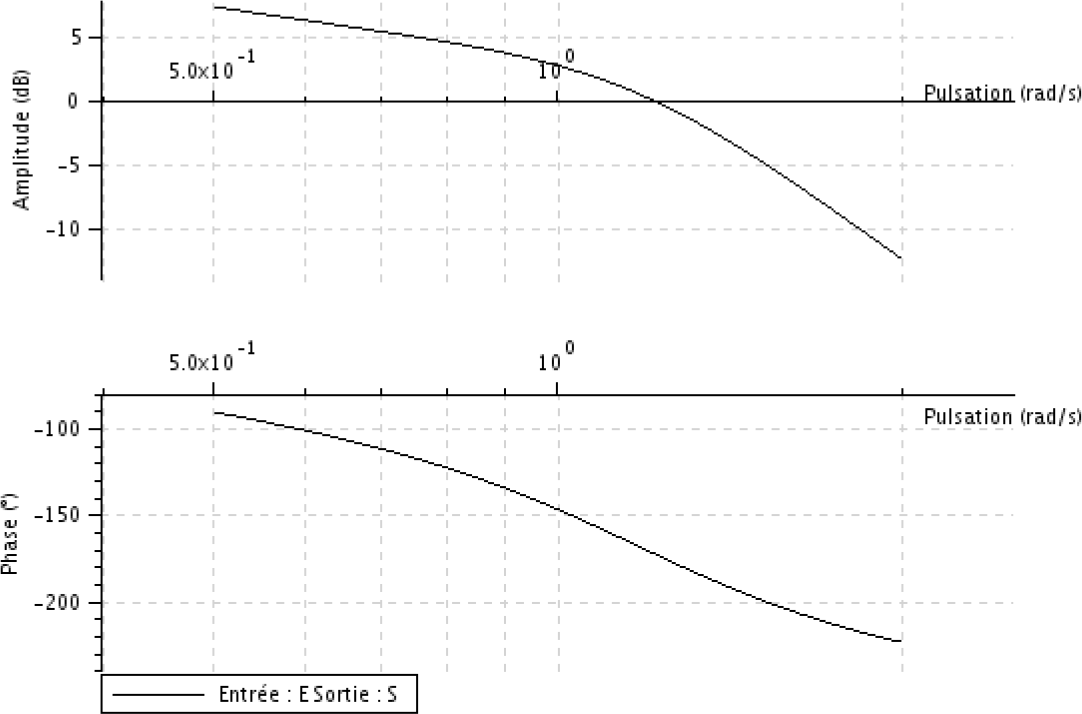
\includegraphics[width=\linewidth]{029_02}
\end{center}


\subparagraph{}\textit{Compléter le câblage du circuit hydraulique à partir du signe « * », ainsi que le schéma du servo-distributeur.}
\ifprof
\begin{corrige}
\end{corrige}
\else
\fi

Au démarrage du véhicule, la valve de décharge du module (b) est fermée. Le distributeur à effet proportionnel (e) est en position médiane, les vérins sont donc immobiles. La commande des vérins est initialement bloquée par une temporisation.

\subparagraph{}\textit{Quelle sont les valeurs des marges de gain et de phase ? }
\ifprof
\begin{corrige}
Les marges de gain et de phase sont très faibles, environ 10\degres de marge de phase et
environ \S{1}{dB} de marge de gain. Elles se
mesurent à des pulsations très proches.
\end{corrige}
\else
\fi


\subparagraph{}\textit{Quelle est la bande passante ?}
\ifprof
\begin{corrige}
La bande passante BP vaut entre 1 et \SI{2}{rad/s},
environ \SI{1,2}{rad/s} par lecture graphique.
\end{corrige}
\else
\fi

\subparagraph{}\textit{Quelle correction proportionnelle $Kp_1$ faut-il choisir pour assurer une bande passante de \SI{0,6}{rad/s} ?}
\ifprof
\begin{corrige}
Le correcteur proportionnel ne modifie pas la phase et translate le gain verticalement de
$20 \log Kp$. Pour assurer une bande passante de \SI{0,6}{rad/s}, il faut que le correcteur baisse la
courbe de gain jusqu'à ce qu'elle croise l'axe \SI{0}{dB} en \SI{0,6}{rad/s}, soit une baisse de$\SI{6}{dB}$
environ, soit $Kp=10^{-\dfrac{6}{20}}=0,5$.
\end{corrige}
\else
\fi

\subparagraph{}\textit{Quelle correction proportionnelle $Kp_2$ faut-il choisir pour assurer une marge de gain de \SI{6}{dB} ?}
\ifprof
\begin{corrige}
La courbe de phase n'étant pas modifiée, la marge de phase est toujours mesurée pour la
même pulsation, là où la phase vaut -180\degres. Avant correction le gain à cette pulsation vaut
environ -1 dB. Pour assurer une marge de gain de \SI{5}{dB}, il faut baisser la courbe de \SI{4}{dB},
soit $Kp=10^{-\dfrac{4}{20}}=0,63$.
\end{corrige}
\else
\fi

\subparagraph{}\textit{Quelle correction proportionnelle $Kp_3$ faut-il choisir pour assurer une marge de phase de
60\degres ?}
\ifprof
\begin{corrige}
Pour assurer une marge de phase de 60\degres, celle-ci doit se mesurer à la pulsation où la phase
vaut $-180+60=-120\degres$, c'est à dire entre 0,7 et \SI{0,8}{rad/s}, \SI{0,78}{rad/s} environ par lecture
graphique. À cette pulsation, le gain vaut avant correction \SI{5}{dB}. Il faut donc descendre la
courbe de $Kp=10^{-\dfrac{5}{20}}=0,566$.
\end{corrige}
\else
\fi

\subparagraph{}\textit{Si le cahier des charges impose une bande passante d'au moins \SI{0,6}{rad/s}, une marge de gain
d'au moins \SI{12}{dB} et une marge de phase d'au moins 60\degres, quelle correction proportionnelle
$Kp$ faut-il choisir ?}
\ifprof
\begin{corrige}
Pour respecter le cahier des charges, il faut $Kp > 0,5$ pour respecter la bande passante et
$Kp<0.63$ et $Kp<0,56$ pour respecter les marges. Toute valeur comprise entre 0,5 et 0,56
convient. Pour optimiser la rapidité, il vaut mieux choisir $Kp=0,56$.
\end{corrige}
\else
\fi
